\date{}
\title{}
\date{}
\begin{document}
\begin{frame}
    \titlepage
\end{frame}


\makeatletter
\newenvironment<>{btHighlight}[1][]
{\begin{onlyenv}#2\begingroup\tikzset{bt@Highlight@par/.style={#1}}\begin{lrbox}{\@tempboxa}}
{\end{lrbox}\bt@HL@box[bt@Highlight@par]{\@tempboxa}\endgroup\end{onlyenv}}

\newcommand<>\btHL[1][]{%
  \only#2{\begin{btHighlight}[#1]\bgroup\aftergroup\bt@HL@endenv}%
}
\def\bt@HL@endenv{%
  \end{btHighlight}%   
  \egroup %
}
\tikzset{
    btHLbox/.style={
        fill=red!30,outer sep=0pt,inner xsep=1pt, inner ysep=0pt, rounded corners=3pt
    },
}
\newcommand{\bt@HL@box}[2][]{%
  \tikz[#1]{%
    \pgfpathrectangle{\pgfpoint{1pt}{0pt}}{\pgfpoint{\wd #2}{\ht #2}}%
    \pgfusepath{use as bounding box}%
    \node[text width={},draw=none,anchor=base west, btHLbox, minimum height=\ht\strutbox+1pt,#1]{\raisebox{1pt}{\strut}\strut\usebox{#2}};
  }%
}

\lst@CCPutMacro
    \lst@ProcessOther {"2A}{%
      \lst@ttfamily 
         {\raisebox{2pt}{*}}% used with ttfamily
         {\raisebox{2pt}{*}}}% used with other fonts
    \@empty\z@\@empty

\lstdefinelanguage
   [x8664gas]{Assembler}     % add a "x64" dialect of Assembler
   [x86masm]{Assembler} % based on the "x86masm" dialect
   % with these extra keywords:
   {morekeywords={CDQE,CQO,CMPSQ,CMPXCHG16B,JRCXZ,LODSQ,MOVSXD,%
                  POPFQ,PUSHFQ,SCASQ,STOSQ,IRETQ,RDTSCP,SWAPGS,.TEXT,.STRING,.ASCIZ,%
                  BEQ,LW,SW,LB,SB,ADDIU,J,BEQZ,BNEZ,BNE,%
                  MOVUPD,MULPD,MOVSD,MULSD,%
                  SHLADD,MOV,CMP.LT,TBIT.NZ,BR.RET.SPTK.MANY,%
                  ADDQ,POPQ,PUSHQ,RRMOVQ,MRMOVQ,RMMOVQ,IRMOVQ,%
                  <-,LL,SC,ADDI,ADDL,VMOVDQA,ADDQ,CMPL,JB,JBE,MOVL,CLTQ,%
                  MOVW,PUSHW,MOV,ADD,SUB,INT,PUSH,MOV,ADD,REP,MOVSB,%
                  TESTQ,CMPQ,MOVL,MOVQ,ADDQ,JMPQ,XORQ,%
                  LEAQ,LEAL,LEA,RETQ,RET,POPL,POPW,PUSHL,PUSHW,%
                  LEAW,%
                  SUBQ,SYSCALL,.ASCII,CALLQ,MOVSLQ,JMP,ANDQ,SHRQ,MOVB,INCQ,TESTL,XORL,%
                  SHRL,LEAL,SARL,SUBL,IMULL,IMULQ,MOVDQU,PADDD,XORL,%
                  MOVZBL,MOVZB,SHRB,SRAL,SHRL,ANDL,%
                  CMOVNS,SRAL,SRAQ,MOVZBW,MOVZBQ,%
                  PADDW,PADDQ,MODUPS,MOVAPD,%
                  MOVL,RET,.GLOBL,%
		  PAUSE,LFENCE,JMP,%
                  },
    deletekeywords={eax,ebx,sp,si,cx,di,ds,cs,es,fs,dx,ax,bx,al,esi,ebp,ecx,rip,eip,edx,edi,rdi,esp},
    deletekeywords=[2]{size},
    alsoletter={\%},
    alsoother={()},
    emphstyle={\color{violet!50!black}},
    emph={\%rax,\%rbx,\%rcx,\%rdx,\%r8,\%r9,\%r10,\%r11,\%r12,\%r13,\%r14,\%r15,\%eax,\%ebx,\%sp,\%si,\%cx,\%di,\%ds,\%cs,\%es,\%fs,\%dx,\%ax,\%bx,\%al,\%esi,\%ebp,\%ecx,\%rip,\%eip,\%edx,\%edi,\%rdi,\%esp,\%rsp},
    %moreemph={eax,ebx,sp,si,cx,di,ds,cs,es,fs,dx,ax,bx,al,esi,ebp,ecx,rip,eip,edx,edi,rdi,esp},
    morecomment=[l]{\#},
    morecomment=[l]{\/\/},
    morecomment=[s]{/*}{*/},
    sensitive=false,
    keepspaces=true} % et

\lstalias[]{myasm}[x8664gas]{Assembler}

\lstdefinelanguage{JavaScript}{
  keywords={typeof, new, true, false, catch, function, return, null, catch, switch, var, if, in, while, do, else, case, break},
  ndkeywords={class, export, boolean, throw, implements, import, this},
  sensitive=false,
  comment=[l]{//},
  morecomment=[s]{/*}{*/},
  morestring=[b]',
  morestring=[b]"
}

\newcommand{\keywordstyle}{\sourcecodeprolight\bfseries\color{blue!30!black}}
\newcommand{\stringstyle}{\color{blue!20!black}\ttfamily}

\lstset{
    language=C,
    basicstyle=\sourcecodepro\EmptyMapping,
    escapechar=`,
    keywordstyle=\keywordstyle\EmptyMapping,
    identifierstyle=\sourcecodepro\EmptyMapping,
    numberstyle=\small\color{black!70},
    commentstyle=\color{red!60!black}\ttfamily\itshape,
    stringstyle=\color{blue!20!black}\ttfamily,
    ndkeywordstyle=\bfseries\color{blue!30!black},
    upquote=true,
}



\lstdefinestyle{medium}{
    basicstyle=\sourcecodepro\EmptyMapping\fontsize{12}{13}\selectfont,
    keywordstyle=\sourcecodepro\EmptyMapping\fontsize{12}{13}\selectfont\keywordstyle,
}

\lstdefinestyle{small}{
    basicstyle=\sourcecodepro\EmptyMapping\small,
    keywordstyle=\sourcecodepro\EmptyMapping\small\keywordstyle,
}

\lstdefinestyle{smaller}{
    basicstyle=\sourcecodepro\EmptyMapping\fontsize{11}{12}\selectfont,
    keywordstyle=\sourcecodepro\EmptyMapping\fontsize{11}{12}\selectfont\keywordstyle,
}

\lstdefinestyle{size105}{
    basicstyle=\sourcecodepro\EmptyMapping\fontsize{10.5}{11.5}\selectfont,
    keywordstyle=\sourcecodepro\EmptyMapping\fontsize{10.5}{11.5}\selectfont\keywordstyle,
}

\lstdefinestyle{size10}{
    basicstyle=\sourcecodepro\EmptyMapping\fontsize{10}{11}\selectfont,
    keywordstyle=\sourcecodepro\EmptyMapping\fontsize{10}{11}\selectfont\keywordstyle,
}

\lstdefinestyle{size9}{
    basicstyle=\sourcecodepro\EmptyMapping\fontsize{9}{10}\selectfont,
    keywordstyle=\sourcecodepro\EmptyMapping\fontsize{9}{10}\selectfont\keywordstyle,
}
\lstdefinestyle{size8}{
    basicstyle=\sourcecodepro\EmptyMapping\fontsize{8}{9}\selectfont,
    keywordstyle=\sourcecodepro\EmptyMapping\fontsize{8}{9}\selectfont\keywordstyle,
}



\lstdefinestyle{script}{
    basicstyle=\sourcecodepro\EmptyMapping\scriptsize,
    keywordstyle=\sourcecodepro\EmptyMapping\scriptsize\bfseries,
}



\usetikzlibrary{arrows.meta,patterns}

\begin{frame}{last time}
    \begin{itemize}
    \item tracing return-oriented programming chains
    \item assembling ROP chains manually
    \item finding gadgets
    \item heuristically finding ROP chians
    \item replacing non-return addresses
        \begin{itemize}
        \item can use `gadgets' to replace function pointers, run other gadget
        \item idea 1: change stack pointer, use ROP chian
        \item idea 2: use chain of jmps/calls
        \end{itemize}
    \item `jump-oriented programming'
    \end{itemize}
\end{frame}

\section{ROP}
\subsection{exercise: ROP alignemnt}



\begin{frame}[fragile]{exercise: ROP chain alignment}
\begin{tikzpicture}
\node (code) {
\begin{lstlisting}[language=C++,style=smaller]
void getInitials(char *init) {
    char first[50]; char second[50];
    scanf("%s%s", first, second);
    init[0] = first[0];
    init[1] = second[0];
}
\end{lstlisting}
};
\node[anchor=north west] (asm) at ([xshift=.2cm]code.north east) {
\begin{lstlisting}[language=myasm,style=smaller]
getInitials: push %rbx
xor    %eax,%eax
mov    %rdi,%rbx
// lea "%s%s" -> %rdi
lea    0xe6e(%rip),%rdi 
sub    $0xa0,%rsp
// &second[0] -> %rdx
lea    0x50(%rsp),%rdx 
// &first[0] -> %rsi
mov    %rsp,%rsi
call   __isoc99_scanf@plt
mov    (%rsp),%al
mov    %al,(%rbx)
mov    0x50(%rsp),%al
mov    %al,0x1(%rbx)
add    $0xa0,%rsp
pop    %rbx
ret 
\end{lstlisting}
};
\node[anchor=north west,align=left,font=\small] at ([yshift=.1cm]code.south west) {
Suppose we have 64-byte ROP chain \\
w/o whitespace in it. How to write input? \\
(Multiple might work) \\
A. \textit{[100 As]}\textit{[ROP chain]} X \\
B. \textit{[44 As]}\textit{[ROP chain]} X \\
C. \textit{[36 As]}\textit{[ROP chain]} X \\
D. \textit{[ROP chain]}\textit{[36 As]}\textit{[ROP chain addr]} X \\
E. X \textit{[42 As]}\textit{[ROP chain]} \\
F. X \textit{[50 As]}\textit{[ROP chain]} \\
G. \textit{[ROP chain]} \textit{[50 As]}\textit{[ROP chain addr]} \\
};
\end{tikzpicture}
\end{frame}



\subsection{exercise: using function pointer overwrite}
\begin{frame}[fragile,label=useFPtrOverwrite1]{using function pointer overwrite (1)}
\begin{lstlisting}[language=C,style=script]
struct Example {
    char input[1000];
    void (*process_function)(Example *, long, char *);
};
void vulnerable(struct Example *e) {
    long index;
    char name[1000];
    gets(e->input); /* can overwrite process_function */
    scanf("%ld,%s", &index, &name[0]); /* expects <decimal number>,<string> */
    (e->process_function)(e /* rdi */, index /* rsi */, name /* rdx */);
}
\end{lstlisting}
\begin{itemize}
\item if we overwrite process\_function's address with the address of the gadget
    \texttt{mov \%rsi, \%rsp; ret}, then the beginning of the input
    should contain\ldots \\
    \begin{itemize}
    \item A. the shellcode to run
    \item B. an ROP chain to run
    \item C. the address of shellcode (or existing function) in decimal
    \item D. the address of the ROP chain to run written out in decimal
    \item E. the address of a RET instruction written out in decimal
    \end{itemize}
\end{itemize}
\end{frame}

\iftoggle{heldback}{\excludecomment{soln}}{\includecomment{soln}}
\begin{soln}
\begin{frame}[fragile,label=useFPtrOverwrite1Explain]{explanation}
\begin{lstlisting}[language=C++,style=script]
gets(e->input); /* can overwrite process_function */
scanf("%ld,%s", &index, &name[0]); /* expects <decimal number>,<string> */
(e->process_function)(e /* rdi */, index /* rsi */, name /* rdx */);
\end{lstlisting}
\texttt{"1234,FOO......."} + addr of \texttt{mov \%rsi, \%rsp, ret}
\begin{itemize}
\item arguments setup registers for gadget:
\begin{itemize}
    \item \%rdi (irrelevant) is "1234,FOO..." (copy in e)
    \item \%rsi is 1234 (from scanf)
    \item \%rdx (irrelevant) is "FOO..." (pointer to name)
\end{itemize}
\item mov in gadget: \%rsi (1234) becomes \%rsp
\item ret in gadget: read pointer at 1234, set \%rsp to 1234 + 8
    \begin{itemize}
    \item jump to next gadget (whose address should be stored at 1234)
    \item if that gadget returns, will read new return address from 1238
    \end{itemize}
\end{itemize}
\end{frame}
\end{soln}

\begin{frame}[fragile,label=useFPtrOverwrite2]{using function pointer overwrite (2)}
\begin{lstlisting}[language=C,style=script]
struct Example {
    char input[1000];
    void (*process_function)(Example *, long, char *);
};
void vulnerable(struct Example *e) {
    long index;
    char name[1000];
    gets(e->input); /* can overwrite process_function */
    scanf("%ld,%s", &index, &name[0]); /* expects <decimal number>,<string> */
    (e->process_function)(e /* rdi */, index /* rsi */, name /* rdx */);
}
\end{lstlisting}
\begin{itemize}
\item if we overwrite process\_function's address with the address of the gadget
    \texttt{push \%rdx; jmp *(\%rdi)}, then the beginning of the input should contain\ldots \\
    \begin{itemize}
    \item A. the shellcode to run
    \item B. an ROP chain to run
    \item C. the address of shellcode (or existing function) 
    \item D. the address of the ROP chain 
    \item E. the address of a RET instruction
    \end{itemize}
\end{itemize}
\end{frame}

\begin{soln}
\begin{frame}[fragile,label=useFPtrOverwrite1Explain]{explanation (one option)}
\begin{lstlisting}[language=C++,style=script]
gets(e->input); /* can overwrite process_function */
scanf("%ld,%s", &index, &name[0]); /* expects <decimal number>,<string> */
(e->process_function)(e /* rdi */, index /* rsi */, name /* rdx */);
\end{lstlisting}
\texttt{"FOOBARBAZ......."} + addr of \texttt{push \%rdx; jmp *(\%rdi)}
\begin{itemize}
\item arguments setup registers for gadget:
\begin{itemize}
    \item \%rdi is "FOOBARBAZ...." (copy in e)
    \item \%rsi (irrelevant) is uninitialized? (scanf failed)
    \item \%rdx (irrelevant) is uninitialized? (scanf failed)
\end{itemize}
\item push in gadget: top of stack becomes copy of uninit. value 
\item jmp in gadget
    \begin{itemize}
    \item interpret ``FOOBARBA'' as 8-byte address
    \item jump to that address
    \end{itemize}
\end{itemize}
\end{frame}

\begin{frame}[fragile,label=useFPtrOverwrite2Explain]{explanation (unlikely alternative?)}
\begin{lstlisting}[language=C++,style=script]
gets(e->input); /* can overwrite process_function */
scanf("%ld,%s", &index, &name[0]); /* expects <decimal number>,<string> */
(e->process_function)(e /* rdi */, index /* rsi */, name /* rdx */);
\end{lstlisting}
\texttt{"1234567890,FOO......."} + addr of \texttt{push \%rdx; jmp *(\%rdi)}
\begin{itemize}
\item arguments setup registers for gadget:
\begin{itemize}
    \item \%rdi is address of string "12345678,FOO..." (copy in e)
    \item \%rsi is 12345678
    \item \%rdx is address of string "FOO..." (copy in name)
\end{itemize}
\item push in gadget: top of stack becomes address of "FOO..."
\item jmp in gadget
    \begin{itemize}
    \item interpret \textit{ASCII encoding of ``12345678''} (???) as 8-byte address
    \item jump to that address
    \end{itemize}
\end{itemize}
\end{frame}
\end{soln}


\subsection{just get rid of rets?}
\begin{frame}{can we get rid of gadgets? (1)}
    \begin{itemize}
    \item Onarlioglu et al, ``G-Free: Defeating Return-Oriented Programming through Gadget-Less Binaries'' (2010)
    \item two parts:
        \begin{itemize}
        \item get rid of unintended jmp, ret instructions
        \item add stack canary-like checks to jmp, ret instructions
        \end{itemize}
    \item hope: no \textit{useful} gadgets b/c of canary-like checks
        \begin{itemize}
        \item all gadgets should be useless without a secret value?
        \item still vulnerable to information leaks
        \end{itemize}
    \item overhead is not low:
        \begin{itemize}
        \item 20--30\% (!) space overhead
        \item 0--6\% time overhead
        \end{itemize}
    \end{itemize}
\end{frame}

\begin{frame}{no unintended jmp/ret (1)}

\includegraphics[width=10cm]{../mitigate/gfree1}
\begin{itemize}
\item \texttt{addl \$0xc2, \%eax}: \texttt{05 \myemph<2>{c2 00 00} 00}
\item problem: \texttt{\myemph<2>{c2 00 00}}: variant of ret instruction
\item paper's proposed fix: change the constant
\end{itemize}
\end{frame}

\begin{frame}{no unintended jmp/ret (2)}
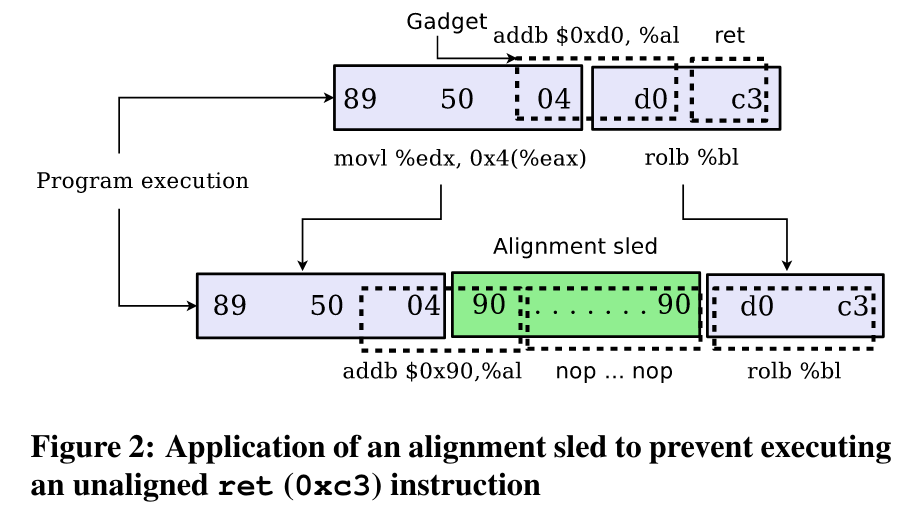
\includegraphics[width=10cm]{../mitigate/gfree2}
\end{frame}


\subsection{other defenses?}
\begin{frame}{other defenses?}
    \begin{itemize}
    \item mentioned shadow stacks
    \vspace{.5cm}
    \item some other ideas later:
    \item pointer authentication
        \begin{itemize}
        \item MACs in return/function/etc. addresses
        \end{itemize}
    \item control flow integrity
        \begin{itemize}
        \item verify that rets go to just after call
        \item verify that calls/jumps/etc. go to intended function/label
        \end{itemize}
    \end{itemize}
\end{frame}


\section{blind ROP}
\begin{frame}{blind ROP}
    \begin{itemize}
    \item \url{https://www.scs.stanford.edu/brop/}
    \end{itemize}
\end{frame}
\begin{frame}{autorestarting servers}
    \begin{itemize}
    \item common strategy for servers:
    \item start server `workers' with same randomization
        \begin{itemize}
        \item fork()'d from common process or
        \item only re-randomized addresses on reboot
        \end{itemize}
    \item automatically restart server workers after crash
    \end{itemize}
\end{frame}

\begin{frame}[fragile]{autorestarting servers [pseudocode]}
\begin{Verbatim}
void vulnerable() {
    char buffer[128];
    read_from_network_into(buffer);
    ...
}

int main() {
    while (true) {
        setup_new_connection();
        run_in_new_process(vulnerable);
    }
}
\end{Verbatim}
\end{frame}

\begin{frame}{a little overwrite (1)}
\begin{tikzpicture}
\coordinate (stack tl) at (0, 0);
\path[draw,thick,fill=yellow!20] (stack tl) ++(0cm, -1cm) coordinate (ra tl) rectangle ++(3.5, -.5)
    coordinate (ra br)
    node [midway] {return address};
\coordinate (ra bl) at (ra tl |- ra br);
\path[draw,thick,fill=violet!20,pattern=north east lines,pattern color=black!20] (ra bl) rectangle ++(3.5, -.5) coordinate (can br)
    node [midway] {stack canary};
\coordinate (can bl) at (ra tl |- can br);
\path[draw,thick,fill=green!20,align=center] (can bl) rectangle ++(3.5, -2)  coordinate (buf br)
    node [midway] {buffer};
\begin{visibleenv}<2->
    \draw[orange,very thick](ra bl) -- ++ (.5cm,0) |- (can br) -- (buf br) -| cycle;
\end{visibleenv}
\begin{scope}[shift={([xshift=1cm,yshift=1cm]ra br)}]
    \begin{visibleenv}<2->
        \node[align=left,anchor=north west] (before-after) at (0, 0) {
            \begin{tabular}{ll}%
            original canary & \tt AB CD EF 01 23 45 67 89 \\%
            after overwrite & \tt ?? CD EF 01 23 45 67 89 \\
            \end{tabular}
        };
    \end{visibleenv}
    \begin{visibleenv}<3->
        \node[align=left,anchor=north west] (outcomes) at (before-after.south west) {
            if {\tt ??}~is {\tt AB}: program works normally \\
            \hspace{.5cm} $\rightarrow$ server gives response \\
            if {\tt ??}~not {\tt AB}: program crashes \\
            \hspace{.5cm} $\rightarrow$ connection closes prematurely  \\
        };
    \end{visibleenv}
    \begin{visibleenv}<4->
        \node[align=left,anchor=north west] (repeat) at ([xshift=-2cm]outcomes.south west) {
            idea: \myemph<4>{keep trying values until it doesn't crash} \\
            if canary not rerandomzied, will find first byte after 256 tries \\
            then \myemph<5>{repeat for every other byte of canary}
        };
    \end{visibleenv}
\end{scope}
\end{tikzpicture}
\end{frame}

\begin{frame}{a little overwrite (2)}
\begin{tikzpicture}
\coordinate (stack tl) at (0, 0);
\path[draw,thick,fill=yellow!20] (stack tl) ++(0cm, -1cm) coordinate (ra tl) rectangle ++(3.5, -.5)
    coordinate (ra br)
    node [midway] {return address};
\coordinate (ra bl) at (ra tl |- ra br);
\path[draw,thick,fill=violet!20,pattern=north east lines,pattern color=black!20] (ra bl) rectangle ++(3.5, -.5) coordinate (can br)
    node [midway] {stack canary};
\coordinate (can bl) at (ra tl |- can br);
\path[draw,thick,fill=green!20,align=center] (can bl) rectangle ++(3.5, -2)  coordinate (buf br)
    node [midway] {buffer};
\begin{visibleenv}<1->
    \draw[orange,very thick](ra bl) -| (can br) -- (buf br) -| cycle;
\end{visibleenv}
\begin{visibleenv}<2->
    \draw[orange,very thick](ra tl) -- ++ (.5cm,0) |- (ra br) -- (buf br) -| cycle;
\end{visibleenv}
\begin{scope}[shift={([xshift=1cm,yshift=1cm]ra br)}]
    \begin{visibleenv}<2->
        \node[align=left,anchor=north west] (before-after) at (0, 0) {
            \begin{tabular}{ll}%
            original return address & \tt 49 43 2A AB 44 00 00 \\%
            after overwrite & \tt ?? 43 2A AB 44 00 00
            \end{tabular}
        };
    \end{visibleenv}
    \begin{visibleenv}<3->
        \node[align=left,anchor=north west] (outcomes) at (before-after.south west) {
            if {\tt ??}~is {\tt 49}: program works normally \\
            \hspace{.5cm} $\rightarrow$ server gives normal response \\
            if {\tt ??}~not {\tt 49}: program does something wierd \\
            \hspace{.5cm} $\rightarrow$ probably weird response \\
        };
    \end{visibleenv}
    \begin{visibleenv}<4->
        \node[align=left,anchor=north west] (repeat) at ([xshift=-2cm]outcomes.south west) {
            can use this to `break' ASLR \\
            find return address value with good confidence
        };
    \end{visibleenv}
\end{scope}
\end{tikzpicture}
\end{frame}

\begin{frame}{blind ROP concept}
    \begin{itemize}
    \item once we know stack canary + return address value
    \item we can guess where program code is
        \begin{itemize}
        \item it's around where the vulnerable is returning to normally
        \end{itemize}
    \vspace{.5cm}
    \item can try replacing return address with nearby addresses
    \item \ldots and see what it does
    \item turns out --- can exploit program \myemph{without access to executable}
    \end{itemize}
\end{frame}

\begin{frame}{blind ROP}
    \begin{itemize}
    \item so far: seems like we need executable to do ROP
    \item \ldots turns out, not really
    \vspace{.5cm}
    \item example attack scenario:
        \begin{itemize}
        \item stack canaries + ASLR + write XOR execute in use
        \item server that's automatically restarted on crash
        \item \ldots and as same randomization every time (fork, what Windows does)
        \end{itemize}
    \end{itemize}
\end{frame}

\begin{frame}{blind canary leaking}
    \begin{itemize}
    \item let's say we have stack overflow:
        \begin{itemize}
        \item [buffer we can overwrite][stack canary][return address]
        \end{itemize}
    \item if we overwrite 0x43 into first byte of stack canary and it doesn't crash\ldots
    \item \ldots then first byte of stack canary was 0x43
    \item if we overwrite 0x43 into first byte + 0x58 in second and it doesn't crash\ldots
    \item \ldots then first+second byte of stack canary was 0x43 + 0x58
    \item can use this to read stack canary
        \begin{itemize}
        \item approx 128 attempts per byte = 1024 trials for 8-byte stack canary
        \end{itemize}
    \end{itemize}
\end{frame}

\begin{frame}{blind return address leaking}
    \begin{itemize}
    \item can use same idea to leak return address (byte-by-byte)
    \item know other interesting addresses are nearby
    \vspace{.5cm}
    \item by guessing addresses find:
        \begin{itemize}
        \item `stop' gadget --- hang program
        \item `crash' gadget --- close connection prematurely
        \end{itemize}
    \end{itemize}
\end{frame}



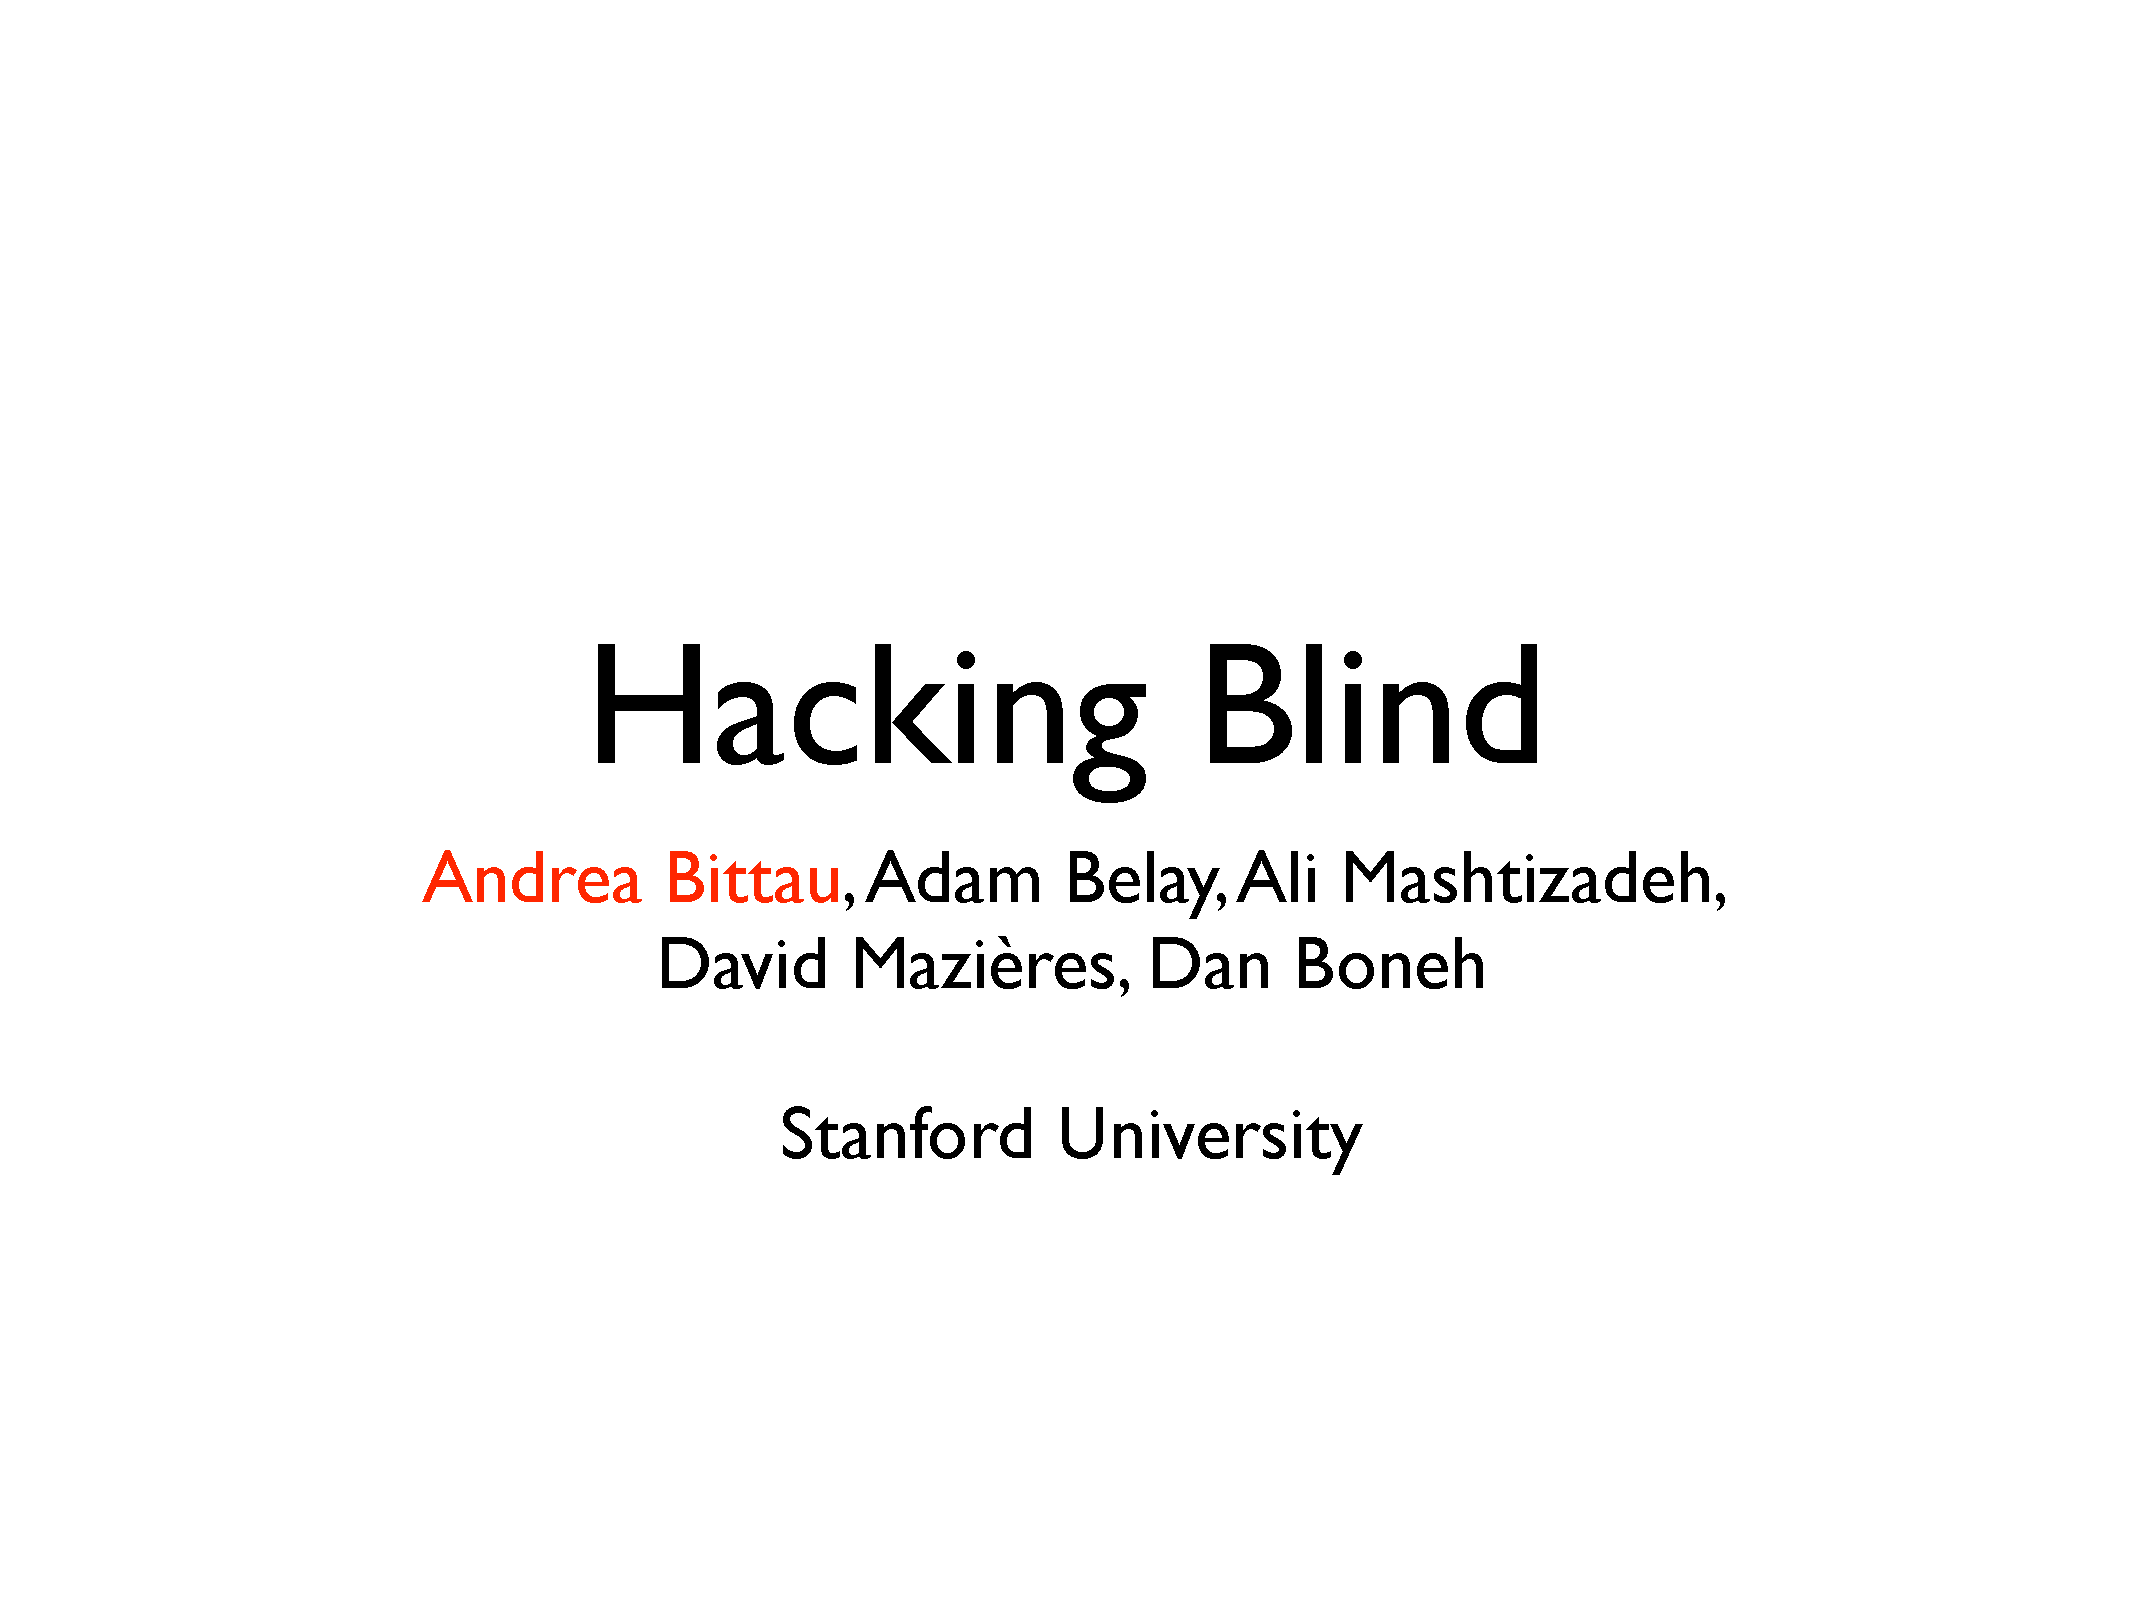
\includepdf[pages=-]{bittau-brop-slides}


% FIXME: blind ROP?
%\includepdf

\usetikzlibrary{calc}

\section{adding bounds checking}
\begin{frame}{so far}
    \begin{itemize}
    \item many vulnerabilities we looked at due to poor bounds checking
        \begin{itemize}
        \item one exception: use-after-free and related
        \end{itemize}
    \vspace{.5cm}
    \item can we just fix this?
    \end{itemize}
\end{frame}


\subsection{compiler-added?}

\begin{frame}[fragile,label=fortifyMemCpyIntro]{adding bounds checking}
\lstset{language=C,style=small}
\begin{lstlisting}
char buffer[42];
memcpy(buffer, attacker_controlled, len);
\end{lstlisting}
    \begin{itemize}
        \item couldn't compiler add check for \texttt{len}
        \item modern Linux: it does
    \end{itemize}
\end{frame}

\begin{frame}[fragile,label=boundsChecking]{added bounds checking}
\lstset{language=C,style=small}
\begin{lstlisting}
char buffer[42];
memcpy(buffer, attacker_controlled, len);
\end{lstlisting}
\lstset{language=myasm,style=small}
\begin{lstlisting}
    subq   $72, %rsp
    leaq   4(%rsp), %rdi
    movslq len, %rdx
    movq   attacker_controlled, %rsi
    movl   $42, %ecx
    call   __memcpy_chk
\end{lstlisting}
    \begin{itemize}
        \item length \texttt{42} passed to \texttt{\_\_memcpy\_chk}
    \end{itemize}
\end{frame}

\begin{frame}{\_FORTIFY\_SOURCE}
    \begin{itemize}
        \item Linux C standard library + GCC features
        \item adds automatic checking to a bunch of string/array functions
        \item also printf (disable \texttt{\%n} unless format string is a constant)
        \vspace{.5cm}
        \item often enabled by default
        \item GCC options:
            \begin{itemize}
                \item \texttt{-D\_FORTIFY\_SOURCE=1} --- enable (backwards-compatible only)
                \item \texttt{-D\_FORTIFY\_SOURCE=2} --- enable (constant sizes only)
                \item \texttt{-D\_FORTIFY\_SOURCE=3} --- enable (computed sizes, sometimes)
                \item \texttt{-U\_FORTIFY\_SOURCE} --- disable
            \end{itemize}
    \end{itemize}
\end{frame}


\begin{frame}[fragile,label=fortifySrcExample]{bounds checking will happen...}
will add checks (gcc 9.3 \textbf{-O2}, FORTIFY\_SOURCE=1/2)
\begin{lstlisting}[language=C,style=smaller]
void example1() {
    char dest1[1024]; memcpy(dest1, ...); ...
}
char dest2[1024];
void example2() {
    memcpy(dest2, ...); ...
}
void example3() {
    char *p = &dest2[4]; memcpy(p, ...); ...
}
\end{lstlisting}
\end{frame}

\begin{frame}[fragile,label=fortifySrcExample2]{bounds checking will happen...}
will add checks (gcc 14.2 or clang 20 \textbf{-Os}, FORTIFY\_SOURCE=3)
\begin{lstlisting}[language=C,style=smaller]
char dest2[1024];
void example4() {
    char *p = &dest2[mystery()]; memcpy(p, ...); ...
}
\end{lstlisting}
\begin{itemize}
\item no checking with FORTIFY\_SOURCE=2
\item extra overhead: computing min(50, 1024-mystery())
\end{itemize}
\end{frame}

\begin{frame}[fragile,label=fortifySrcExample3]{bounds checking will happen...}
will add check (gcc 14.2 or clang 20 \textbf{-Os}, FORTIFY\_SOURCE=3)
\begin{lstlisting}[language=C,style=smaller]
char dest2[1024];
void example5() {
    char dest3[128];
    char *p = dest2;
    if (mystery()) p = dest3;
    memcpy(p, ...); ...
}
\end{lstlisting}
\begin{itemize}
\item checks for maximum possible with FORTIFY\_SOURCE=2
\end{itemize}
\end{frame}

\begin{frame}[fragile,label=fortifySourceExample4]{bounds checking won't happen...}
\begin{lstlisting}[language=C,style=smaller]
char dest2[1024];
struct Foo {
    char buffer1[128];
    int *pointer;
    ...
};
void example6(struct Foo *f, int size) {
    memcpy(f->buffer1, dest2, size);
}
\end{lstlisting}
\end{frame}

\begin{frame}[fragile,label=fortifySourceExample4]{bounds checking won't quite happen...}
\begin{lstlisting}[language=C,style=smaller]
char dest2[1024];
struct Foo {
    char buffer1[128];
    int *pointer;
    ...
};
struct Foo f;
void example6(int size) {
    memcpy(f.buffer1, dest2, size);
}
\end{lstlisting}
\begin{itemize}
\item checks that size is less than sizeof(struct Foo) (not 128)
\end{itemize}
\end{frame}

\begin{frame}{implementation}
    \begin{itemize}
    \item GCC/clang expose `object size` and `dynamic object size' function
    \item relies on compiler analysis to know size from see declaration or malloc/etc. assignemnt
    \vspace{.5cm}
    \item limited
    \end{itemize}
\end{frame}

\subsection{and library functions}
        % FIXME: exercise: what should call have been
            % needs answers

\begin{frame}[fragile,label=nonChecking]{non-checking library functions}
\lstset{language=C,style=small}
    \begin{itemize}
    \item some C library functions make bounds checking hard: 
\begin{lstlisting}
strcpy(dest, source);
strcat(dest, source);
sprintf(dest, format, ...);
\end{lstlisting}
    \item bounds-checking versions (\myemph{added to library later}):
\begin{lstlisting}
/* might not add \0 (!) */
strncpy(dest, source, size);
strncat(dest, source, size);
snprintf(dest, size, format, ...);
\end{lstlisting}
    \end{itemize}
\end{frame}

\begin{frame}[fragile,label=poorBoundsChecking]{poor bounds-checking APIs}
\begin{lstlisting}[language=C,style=smaller]
char dest[100];
/* THIS CODE IS BROKEN */
strncpy(dest, source1, sizeof dest);
strncat(dest, source2, sizeof dest);
printf("result was %s\n", dest)
\end{lstlisting}
\begin{itemize}
\item the above can access memory of out of bounds
\item \ldots in a bunch of ways
\end{itemize}
\end{frame}

\begin{frame}[fragile,label=strncpyManual]{Linux's strncpy manual}
\begin{lstlisting}[language=C,style=smaller]
strncpy(dest, source1, sizeof dest);
\end{lstlisting}
\begin{itemize}
\item ``Warning: If there is no
       null byte among the first n bytes of src, the string placed in dest will not be null-terminated.''
\end{itemize}
\begin{itemize}
\item exercise: what should the call have been?
\end{itemize}
\end{frame}


\begin{frame}[fragile,label=strncatManual]{Linux's strncat manual}
\begin{lstlisting}[language=C,style=smaller]
strncat(dest, source2, sizeof dest);
\end{lstlisting}
\begin{itemize}
\item ``If src contains n or more bytes, strncat() writes n+1 bytes to  dest  (n
from  src  plus the terminating null byte).  Therefore, the size of dest
must be at least strlen(dest)+n+1.''
\end{itemize}
\begin{itemize}
\item exercise: what should the call have been?
\end{itemize}
\end{frame}

\begin{frame}[fragile,label=betterStrX]{better versions?}
\begin{itemize}
\item FreeBSD (and Linux via libbsd): strlcpy, strlcat
\item ``Unlike [strncat and strncpy], strlcpy() and strlcat() take the full size of the buffer
        and gaurenteeto NUL-terminate the result...''
\end{itemize}
\begin{lstlisting}[language=C++,style=smaller]
strlcpy(dest, source1, sizeof dest);
strlcat(dest, source2, sizeof dest);
\end{lstlisting}
\vspace{.5cm}
\begin{itemize}
\item Windows: \texttt{strcpy\_s}, \texttt{strcat\_s} (same idea, differentname)
\end{itemize}
\end{frame}

\begin{frame}[fragile,label=cppBounds]{C++/Rust bounds checking}
\lstset{language=C,style=small}
\begin{lstlisting}
#include <vector>
...
std::vector<int> data;
data.resize(50);
// undefined behavior:
data[60] = 0;
// throws std::out_of_range exception
data.at(60) = 0;
\end{lstlisting}
\vspace{-\baselineskip}
\hrulefill
\begin{Verbatim}[fontsize=\small]
let data: Vec<i32> = ...;
data.resize(50, 0);
// undefined behavior:
unsafe { *data.get_unchecked_mut(60) = 1; }
// panics at runtime:
data[60] = 0;  
\end{Verbatim}
\end{frame}



\subsection{language support?}


\begin{frame}{language-level solutions}
    \begin{itemize}
    \item languages like Python don't have this problem
    \item couldn't we do the same thing in C?
    \end{itemize}
\end{frame}




\subsection{simple case for bounds checking in C}
\begin{frame}{bounds-checking C}
    \begin{itemize}
    \item there have been many proposals to add bounds-checking to C
    \item including implementations
    \item brainstorm: \myemph{why hasn't this happened?}
    \end{itemize}
\end{frame}

\begin{frame}[fragile,label=addBounds]{easy bounds-checking}
    \lstset{language=C,style=smaller}
\begin{lstlisting}
void vulnerable() {
    char buffer[100];
    int c;
    int i = 0;
    while ((c = getchar()) != EOF && c != '\n') {
        buffer[i] = c;
    }
}
void vulnerable_checked() {
    char buffer[100];
    int c;
    int i = 0;
    while ((c = getchar()) != EOF && c != '\n') {
        FAIL_IF(i >= 100 || i < 0);
        buffer[i] = c;
    }
}
\end{lstlisting}
\end{frame}


\subsection{the problematic case}
\begin{frame}[fragile,label=addBoundsHarder]{harder bounds-checking}
    \lstset{language=C,style=smaller}
\begin{lstlisting}
void vulnerable(char *buffer) {
    char buffer[100];
    int c;
    int i = 0;
    while ((c = getchar()) != EOF && c != '\n') {
        buffer[i] = c;
    }
}
void vulnerable_checked(char *buffer) {
    int c;
    int i = 0;
    while ((c = getchar()) != EOF && c != '\n') {
        FAIL_IF(i >= UNKNOWN || i < UNKNOWN);
        buffer[i] = c;
    }
}
\end{lstlisting}
\end{frame}


\subsection{fat pointer idea}
% FIXME: smoother transition
    % FIXME: exercise about problematic cases


\begin{frame}[fragile,label=wrappedPointers]{adding bounds-checking --- fat pointers}
\lstset{
    language=C,
    style=small
}
\begin{lstlisting}
struct MyPtr {
    char *pointer; /* "raw" pointer value */
    char *minimum; /* first byte of buffer pointed to */
    char *maximum; /* last byte of buffer pointed to */
};
\end{lstlisting}
\begin{visibleenv}<2->
\hrule
\begin{lstlisting}
char buffer[100];
char *p = &buffer[10];
\end{lstlisting}
becomes
\begin{lstlisting}
char buffer[100];
MyPtr p = {
    .pointer = &buffer[10],
    .minimum = &buffer[0],
    .maximum = &buffer[99]
};
\end{lstlisting}
\end{visibleenv}
\end{frame}



\subsubsection{strcpy example}
\begin{frame}[fragile,label=wrappedPtrStrcpy]{adding bounds checking --- strcpy}
\lstset{
    language=C,
    style=small
}
\begin{lstlisting}
MyPtr strcpy(MyPtr dest, const MyPtr src) {
    int i;
    do {
        CHECK(src.pointer + i <= src.maximum);
        CHECK(src.pointer + i >= src.minimum);
        CHECK(dest.pointer + i <= dest.maximum);
        CHECK(dest.pointer + i >= dest.minimum);
        dest.pointer[i] = src.pointer[i];
        i += 1;
        CHECK(src.pointer + i <= src.maximum);
        CHECK(src.pointer + i >= src.minimum);
    } while (src.pointer[i] != '\0');
    return dest;
}
\end{lstlisting}
\end{frame}




\subsubsection{overhead?}

\begin{frame}{speed of bounds checking}
    \begin{itemize}
    \item two comparisons for every pointer access?
    \item three times as much space for every pointer?
    \end{itemize}
\end{frame}



\subsection{unfortunate things C programmers do}
\begin{frame}[fragile,label=unfortunateCProg1]{unfortunate things C programmers do (1)}
from FreeBSD's bootpd (server for machines that boot from the network):
\begin{lstlisting}[language=C,style=smaller]
struct shared_string {
    unsigned int linkcount;
    char         string[1]; /* Dynamically extended */
};
...
s = (struct shared_string *) smalloc(
        sizeof(struct shared_string) + length
    );
...
\end{lstlisting}
\end{frame}

\begin{frame}[fragile,label=unfortunateCProg2]{unfortunate things C programmers do (2)}
from perl's source code:
\begin{lstlisting}[language=C,style=small]
sv_setuv(my_pool_sv, PTR2UV(my_poolp));
...
/* later, in another function: */
my_pool_t *my_poolp = INT2PTR(my_pool_t*, SvUV(my_pool_sv));
\end{lstlisting}
\begin{itemize}
\item PTR2UV: pointer to Unsigned int Value
\item INT2PTR: integer to pointer value
\end{itemize}
\end{frame}

\begin{frame}[fragile,label=unfortunateCProg3]{unfortunate things C programmers do (3)}
\begin{lstlisting}[language=C,style=small]
struct SuperClass;
struct SubClass {
    struct SuperClass super;
    ...
}

struct SubClass sub;
struct SuperClass *super = &sub.super;
some_function(super);
...
some_function(struct SuperClass *super) {
    ...
    struct SubClass *sub = (struct SubClass *)super;
    ...
}
\end{lstlisting}
\end{frame}



\subsection{fat pointers in reality?}
\begin{frame}{example: CCured}
\begin{itemize}
\item Necula et al, ``CCured:  Type-Safe Retrofitting of Legacy Code'' (2002)
\vspace{.5cm}
\item extension to C to add fat pointers
\item actually three different types of pointers:   
    \begin{itemize}
    \item SAFE: point to single object (not array) or NULL
    \item SEQUENCE: pointer to array with known bounds (like ``fat'' pointers)
    \item DYNAMIC: extra to handles type-casting
    \end{itemize}
\item \textit{needs source changes} to annotate some pointer usage
    \begin{itemize}
    \item especially to allow library function calls
    \end{itemize}
\item 1-\textbf{2.5x} time overhead
\end{itemize}
\end{frame}


\section{baggy bounds checking}

\begin{frame}{research example (2009)}
    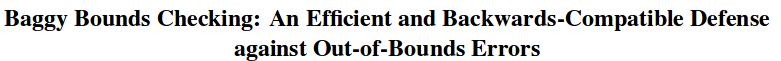
\includegraphics[width=\textwidth]{../bounds/baggy-bounds-title}
\end{frame}

\begin{frame}[fragile,label=lookupTable]{baggy bounds checking idea}
    \begin{itemize}
        \item giant lookup table --- one entry for every 16 bytes of memory
        \item table indicates start of object allocated here
        \item check pointer arithmetic:
    \end{itemize}
\begin{lstlisting}
char p = str[i];
/* becomes: */
CHECK(START_OF[str / 16] == START_OF[&str[i] / 16]);
char p = str[i];
\end{lstlisting}
\end{frame}




\subsection{trick for good performance}

\begin{frame}[fragile,label=baggyBoundsTrick]{baggy bounds trick}
\lstset{language=C,style=small}
    \begin{itemize}
        \item table of pointers to starting locations would be huge
        \item add some restrictions:
            \begin{itemize}
            \item all object sizes are powers of two
            \item all object starting addresses are a multiple of their size
            \end{itemize}
        \item then, table contains size info only:
            \begin{itemize}
            \item table contains $i$, size is $2^i$ bytes:
            \end{itemize}
    \end{itemize}
\begin{lstlisting}
char *GetStartOfObject(char *pointer) {
    return pointer & ~(1 << TABLE[pointer / 16] - 1);
    /* pointer bitwise-and 2^(table entry) - 1 */
    /* clear lower (table entry) bits  of pointer */
}
\end{lstlisting}
\end{frame}



\subsection{the lookup table}
\usetikzlibrary{fit,matrix}

\tikzset{
    stackBox/.style={very thick},
    allocBox/.style={dashed,very thick,fill=blue!20},
    onStack/.style={thick},
    frameOne/.style={fill=blue!15},
    frameTwo/.style={fill=red!15},
    markLine/.style={blue!50!black},
    markLineB/.style={red!90!black},
    hiLine/.style={red!90!black},
}
\begin{frame}<1-6>[fragile,label=lkpTble]{allocations and lookup table}
    \begin{tikzpicture}
        \draw[onStack] (0, 0) rectangle (4, -7);
        \draw[allocBox] (0, 0) rectangle (4, -0.4);
        \draw[stackBox] (0, 0) rectangle (4, -0.5);
        \draw[allocBox] (0, -0.5) rectangle (4, -0.8);
        \draw[stackBox] (0, -0.5) rectangle (4, -1.0);
        \draw[allocBox] (0, -1) rectangle (4, -1.9);
        \draw[stackBox] (0, -1) rectangle (4, -2);
        \draw[allocBox] (0, -2) rectangle (4, -2.4);
        \draw[stackBox] (0, -2) rectangle (4, -2.5);
        \draw[allocBox] (0, -2.5) rectangle (4, -2.7);
        \draw[stackBox] (0, -2.5) rectangle (4, -3);
        \draw[stackBox] (0, -3) rectangle (4, -4);
        \draw[allocBox] (0, -4) rectangle (4, -5.2);
        \draw[stackBox] (0, -4) rectangle (4, -6);

        \begin{visibleenv}<1->
            \node[anchor=north west,align=left] at (9, 0) {
                object allocated in \\ \myemph<1>{power-of-two `slots'}
            };
        \end{visibleenv}
        \begin{visibleenv}<2->
            \matrix[tight matrix,
                nodes={text width=1cm,font=\small\tt},anchor=north west,label={north:table}] (tbl) at (7, -1) {
                $2^4$ \\ $2^4$  \\ $2^5$ \\ $2^5$ \\ $2^4$ \\ $2^4$ \\
                $0$ \\ $0$ \\
                $2^6$ \\ $2^6$ \\ $2^6$ \\ $2^6$ \\
            };
            \begin{scope}[thick,dotted,-Latex]
            \draw (4, -.25) -- (tbl-1-1.west);
            \draw (4, -.75) -- (tbl-2-1.west);
            \draw (4, -1.25) -- (tbl-3-1.west);
            \draw (4, -1.75) -- (tbl-4-1.west);
            \draw (4, -2.25) -- (tbl-5-1.west);
            \draw (4, -2.75) -- (tbl-6-1.west);
            \draw (4, -3.25) -- (tbl-7-1.west);
            \draw (4, -3.75) -- (tbl-8-1.west);
            \draw (4, -4.25) -- (tbl-9-1.west);
            \end{scope}
        \end{visibleenv}
        \begin{visibleenv}<3>
            \draw[ultra thick,red] (0, -1) rectangle (4, -2);
            \node[draw,ultra thick,red,inner sep=0mm,fit=(tbl-3-1) (tbl-4-1)] {};
            \draw[ultra thick,blue] (0, -4) rectangle (4, -6);
            \node[draw,ultra thick,blue,inner sep=0mm,fit=(tbl-9-1) (tbl-12-1)] {};
        \end{visibleenv}
        \begin{visibleenv}<3->
            \node[anchor=north west,align=left] at (9, -2) {
                table stores sizes \\
                \myemph{for each 16 bytes}
            };
        \end{visibleenv}
        \begin{visibleenv}<4>
            \draw[ultra thick,red] (0, -3) rectangle (4, -4);
            \node[draw,ultra thick,red,inner sep=0mm,fit=(tbl-7-1) (tbl-8-1)] {};
        \end{visibleenv}
        \begin{visibleenv}<4->
            \node[anchor=north west,align=left] at (9, -3.5) {
                addresses \textbf<4>{multiples of size} \\
                (may \myemph{require padding})
            };
        \end{visibleenv}
        \begin{pgfonlayer}{bg}
        \begin{visibleenv}<5>
            \fill[red!30] (0, -5.2) rectangle (4, -6.);
            \fill[red!30] (0, -2.7) rectangle (4, -3.);
            \fill[red!30] (0, -1.9) rectangle (4, -2.);
            \fill[red!30] (0, -2.4) rectangle (4, -2.5);
            \fill[red!30] (0, -0.8) rectangle (4, -1.);
            \fill[red!30] (0, -0.4) rectangle (4, -0.5);
        \end{visibleenv}
        \end{pgfonlayer}
        \begin{visibleenv}<5->
            \node[anchor=north west,align=left] at (9, -5.5) {
                sizes are \textbf<5>{powers of two} \\
                (may \myemph{require padding})
            };
        \end{visibleenv}
    \end{tikzpicture}
\end{frame}

\begin{frame}[fragile,label=managing]{managing the table}
    \begin{itemize}
        \item not just done \texttt{malloc()/new}
        \item also for stack allocations:
    \end{itemize}
    \begin{lstlisting}[style=small,language=C]
void vulnerable() {
    char buffer[100];
    gets(vulnerable);
}
\end{lstlisting}
    \begin{tikzpicture}[remember picture, overlay]
        \node[anchor=north east] at ([xshift=-.25cm, yshift=-1cm]current page.north east) {
    \begin{lstlisting}[style=small,language=myasm]
vulnerable:
  // make %rsp a multiple
  // of 128 (2^7) 
  andq $0xFFFFFFFFFFFFFF80, %rsp
  // allocate 128 bytes
  subq $0x80, %rsp
  // rax <- rsp / 16
  movq $rsp, %rax
  shrq $4, %rax
  movb $7, TABLE(%rax)
  movb $7, TABLE+1(%rax)
  ...
  movq %rsp, %rdi
  call gets
  ret
\end{lstlisting}
};
    \end{tikzpicture}
\end{frame}

\begin{frame}[fragile,label=sparseLookup]{sparse lookup table}
    \begin{tikzpicture}
        \node[anchor=south] at (3.5, 3) {lookup table};
        \draw[stackBox] (0, 3) rectangle (7, -3);
        \draw[pattern color=red,pattern=north west lines,onStack] (0, -3) rectangle (7, -1.5)
            node[midway,fill=white,align=center] {unallocated memory (segfault) };
        \draw[fill=green,onStack] (0, -1.5) rectangle (7, .2)
            node[midway] { allocated part of table };
        \draw[pattern color=red,pattern=north west lines,onStack] (0, .20) rectangle (7, 1.3)
            node[midway,fill=white,align=center] {unallocated memory (segfault) };
        \draw[fill=green,onStack] (0, 1.3) rectangle (7, 1.6);
        \draw[pattern color=red,pattern=north west lines,onStack] (0, 1.6) rectangle (7, 2.3);
        \draw[fill=green,onStack] (0, 2.3) rectangle (7, 3)
            node[midway] { allocated part of table };
    \end{tikzpicture}
\end{frame}



\subsection{checks using table}
\usetikzlibrary{calc}
\begin{frame}{baggy bounds check: added code}
    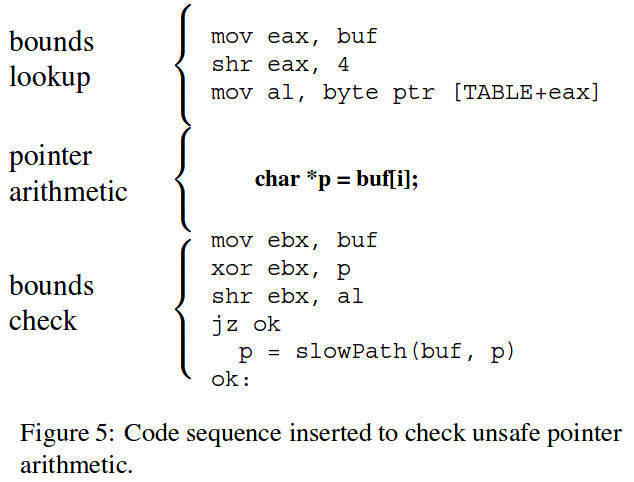
\includegraphics[width=0.6\textwidth]{../bounds/bb-bounds-check}
\end{frame}

\begin{frame}[fragile,label=addedCode]{baggy bounds check: added code}
    \lstset{language=myasm,style=small}
    \begin{lstlisting}
/* bounds lookup */
    mov buf, %rax
    shr %rax, 4
    mov LOOKUP_TABLE(%rax), %al
/* array element address computation */
    ...    // `\textbf{\textit{char * p = buf[i];}}`
/* bound check */
    mov buf, %rbx
    xor p, %rbx
    shr %al, %rbx
    jz  ok
    ...    // handle possible violation
ok:
\end{lstlisting}

    \imagecredit{adapted from paper figure}
\end{frame}

\begin{frame}{avoiding checks}
    \begin{itemize}
        \item code not added if not array/pointer accesses to object
        \item code not added when pointer accesses ``obviously'' safe
            \begin{itemize}
            \item author's implementation: only checked within function
            \end{itemize}
    \end{itemize}
\end{frame}



\subsection{exercise: overhead estimating?}
\begin{frame}<1>[fragile,label=bbOverheadExer1]{exercise: overhead of baggy bounds (1)}
\begin{itemize}
\item suppose program allocates:
    \begin{itemize}
    \item 1000 100 byte objects
    \item 1 10000 byte object
    \end{itemize}
\item using baggy bounds, estimate:
    \begin{itemize}
    \item space required for padding
        \begin{itemize}
        \item<2-> $(128-100)\cdot 1000 + (16384 - 10000)) = 34384$
        \end{itemize}
    \item space required for table
        \begin{itemize}
        \item<2-> $(128\cdot 1000 + 16384) \div 16 = 9024$
        \end{itemize}
    \end{itemize}
\end{itemize}
\end{frame}

\iftoggle{heldback}{}{\againframe<2>{bbOverheadExer1}}

\begin{frame}[fragile,label=bbOverheadExer2]{exercise: overhead of baggy bounds (2)}
\begin{lstlisting}[language=C,style=smaller]
char *strcat(char *d, char *s) {
    int i;
    for (i = 0; s[i] != '\0'; i += 1) {
        d[i] = s[i]; 
    }
    d[i] = '\0';
    return d;
}
\end{lstlisting}
\begin{itemize}
\item estimate:
\begin{itemize}
\item number of bounds checks needed
\item very rough number of instructions run w/o bounds check
\end{itemize}
\item thought question: \\
with bounds checking, what's fastest possible code?
\end{itemize}
\end{frame}


\subsection{alternative: pointer tagging}

\begin{frame}{alternate approach: pointer tagging}
    \begin{itemize}
        \item some bits of \myemph{address} are size 
        \begin{itemize}
        \item replaces table entry/lookup
        \end{itemize}
    \item change code to allocate objects this way
    \item works well on 64-bit --- plenty of addresses to use
    \end{itemize}
    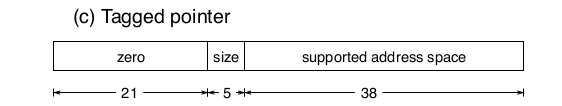
\includegraphics[width=0.8\textwidth]{../bounds/baggy-bounds-tagging}
\end{frame}



\subsection{performance?}

\begin{frame}{baggy bounds performance}
    \begin{itemize}
        \item table: 4--72\% time overhead (depends on benchmark suite)
        \item table: 11--21\% space overhead (depends on benchmark suite)
        \item tagged pointers: slightly better on average
    \end{itemize}
\end{frame}

\begin{frame}{baggy bounds performance}
    \begin{center}
    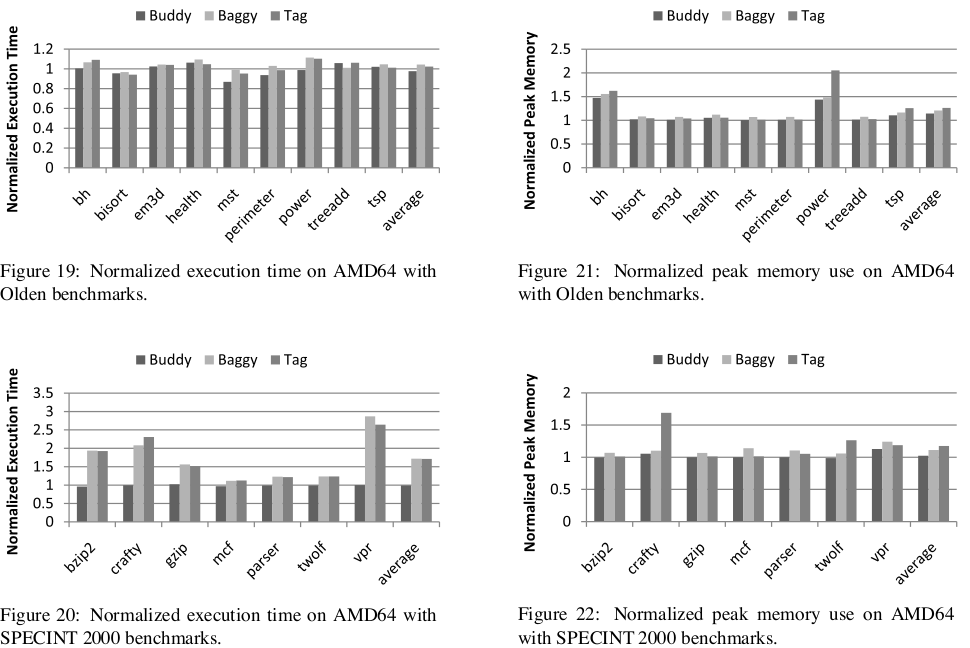
\includegraphics[height=0.8\textheight]{../bounds/baggy-bounds-perf}
    \end{center}
\end{frame}



\subsection{problem: pointers within objects}
% FIXME
\begin{frame}[fragile,label=withinObj]{problem: within object}
\begin{lstlisting}
struct foo {
    char buffer[1024];
    int *pointer;
};
struct foo array_of_foos[1024];
...
char *p = &array_of_foos[4].buffer[4]
\end{lstlisting}
\begin{itemize}
\item exercise: what are the bounds for p?
\end{itemize}
\end{frame}


\subsection{corner cases}

\begin{frame}[fragile,label=unfortunateCProgF2C]{unfortunate things C programmers do (4)}
in code generated by f2c (Fortran to C translator) \\
{\scriptsize (cleaned up slightly)}
\begin{lstlisting}[language=C,style=small]
float sum(int size, float *arr) {
    arr = arr - 1; /* <-- deliberately out-of-bounds pointer */
    float result = 0.f;
    for (i = 1; i <= size; ++i) {
        result += arr[i]
    }
    return result;
}
\end{lstlisting}
\end{frame}



\section{AddressSanitizer}

\begin{frame}{AddressSanitizer}
    \begin{itemize}
    \item like baggy bounds:
        \begin{itemize}
        \item big lookup table
        \item lookup table set by memory allocations
        \item compiler modification: change stack allocations
        \end{itemize}
    \item unlike baggy bounds:
        \begin{itemize}
        \item check reads/writes (instead of pointer computations)
        \item only detect errors that read/write \myemph{between objects}
        \item object sizes not padded to power of two
        \item table has info for every single byte (more precise)
        \end{itemize}
    \end{itemize}
\end{frame}




\subsection{ASan's added check}

\begin{frame}[fragile,label=asanVBounds]{adding bounds-checking example}
\lstset{
    language=C++,
    style=small,
    moredelim={**[is][\btHL<2>]{~2~}{~end~}},
}
\begin{lstlisting}
void vulnerable(long value, int offset) {
    long array[10] = {1,2,3,4,5,6,7,8,9,10};
    // generated code: (added by AddressSanitizer)
    ~2~if (!lookup_table[&array[offset]] == VALID) FAIL();~end~
    array[offset] = value;
    do_something_with(array);
}
\end{lstlisting}
    \begin{itemize}
        \item AddressSanitizer: crashes only if \lstinline|array[offset]| isn't part of any object
            \begin{itemize}
            \item but no extra space --- single-byte precision
            \end{itemize}
    \end{itemize}
\end{frame}



\subsection{stack layout}
\usetikzlibrary{arrows.meta,matrix,patterns}
\tikzset{
    stackBox/.style={very thick},
    allocBox/.style={dashed,very thick,fill=blue!20},
    onStack/.style={thick},
    frameOne/.style={fill=blue!15},
    frameTwo/.style={fill=red!15},
    markLine/.style={blue!50!black},
    markLineB/.style={red!90!black},
    hiLine/.style={red!90!black},
}
\begin{frame}[fragile,label=asanStackLayout]{AddressSanitizer stack layout}
    \begin{tikzpicture}
        \begin{scope}[x=1.7cm]
    \draw[stackBox] (0, 0) rectangle (5, -6);
            \draw[onStack] (0, 0) rectangle (5, -.5)
        node[midway] (arrayLoc) { return address (for \texttt{vulernable()}) };
    \begin{visibleenv}<2>
        \node[anchor=west] at (5.25, -.25) { $\approx$ \tt array[0x13]};
        \node[anchor=west] at (5.25, -3.75) { $\approx$ \tt array[0xa]};
    \end{visibleenv}
    \draw[onStack] (0, -.5) rectangle (5, -1)
        node[midway] { saved \tt\%rbp };
    \draw[onStack] (0, -1) rectangle (5, -1.5)
        node[midway] { saved \tt\%r13 };
    \draw[onStack] (0, -1.5) rectangle (5, -2)
        node[midway] { saved \tt\%r12 };
    \draw[onStack] (0, -2) rectangle (5, -2.5)
        node[midway] { saved \tt\%rbx };
    \draw[onStack,pattern=north west lines,pattern color=red] (0, -2.5) rectangle (5, -4)
        node[midway,fill=white] { ``red zone'' };
    \draw[onStack] (0, -4) rectangle (5, -6)
        node[midway,fill=white] { \tt array };
            \draw[onStack,dashed] (0, -4) rectangle (5, -4.5) node[midway] {\tt array[9]};
            \begin{visibleenv}<3>
            \matrix[tight matrix,
                nodes={text width=3cm,font=\small\tt},anchor=north west,label={north:lookup table}] (tbl) at (6, -2) {
                valid \\ valid  \\ valid \\ valid \\ valid \\ invalid \\ invalid \\
                invalid \\ invalid \\ valid \\ valid \\ \ldots \\
            };
                \draw[thick,-Latex] (5, -.25) -- (tbl-1-1.west);
                \draw[thick,-Latex] (5, -.75) -- (tbl-2-1.west);
            \end{visibleenv}
    \draw[thick,-Latex] (5.15, -6) --++ (0, 2);
        \end{scope}
    \end{tikzpicture}
\end{frame}





\section{AddressSanitizer}

\begin{frame}{AddressSanitizer}
    \begin{itemize}
    \item like baggy bounds:
        \begin{itemize}
        \item big lookup table
        \item lookup table set by memory allocations
        \item compiler modification: change stack allocations
        \end{itemize}
    \item unlike baggy bounds:
        \begin{itemize}
        \item check reads/writes (instead of pointer computations)
        \item only detect errors that read/write \myemph{between objects}
        \item object sizes not padded to power of two
        \item table has info for every single byte (more precise)
        \end{itemize}
    \end{itemize}
\end{frame}




\subsection{ASan's added check}

\begin{frame}[fragile,label=asanVBounds]{adding bounds-checking example}
\lstset{
    language=C++,
    style=small,
    moredelim={**[is][\btHL<2>]{~2~}{~end~}},
}
\begin{lstlisting}
void vulnerable(long value, int offset) {
    long array[10] = {1,2,3,4,5,6,7,8,9,10};
    // generated code: (added by AddressSanitizer)
    ~2~if (!lookup_table[&array[offset]] == VALID) FAIL();~end~
    array[offset] = value;
    do_something_with(array);
}
\end{lstlisting}
    \begin{itemize}
        \item AddressSanitizer: crashes only if \lstinline|array[offset]| isn't part of any object
            \begin{itemize}
            \item but no extra space --- single-byte precision
            \end{itemize}
    \end{itemize}
\end{frame}



\subsection{stack layout}
\usetikzlibrary{arrows.meta,matrix,patterns}
\tikzset{
    stackBox/.style={very thick},
    allocBox/.style={dashed,very thick,fill=blue!20},
    onStack/.style={thick},
    frameOne/.style={fill=blue!15},
    frameTwo/.style={fill=red!15},
    markLine/.style={blue!50!black},
    markLineB/.style={red!90!black},
    hiLine/.style={red!90!black},
}
\begin{frame}[fragile,label=asanStackLayout]{AddressSanitizer stack layout}
    \begin{tikzpicture}
        \begin{scope}[x=1.7cm]
    \draw[stackBox] (0, 0) rectangle (5, -6);
            \draw[onStack] (0, 0) rectangle (5, -.5)
        node[midway] (arrayLoc) { return address (for \texttt{vulernable()}) };
    \begin{visibleenv}<2>
        \node[anchor=west] at (5.25, -.25) { $\approx$ \tt array[0x13]};
        \node[anchor=west] at (5.25, -3.75) { $\approx$ \tt array[0xa]};
    \end{visibleenv}
    \draw[onStack] (0, -.5) rectangle (5, -1)
        node[midway] { saved \tt\%rbp };
    \draw[onStack] (0, -1) rectangle (5, -1.5)
        node[midway] { saved \tt\%r13 };
    \draw[onStack] (0, -1.5) rectangle (5, -2)
        node[midway] { saved \tt\%r12 };
    \draw[onStack] (0, -2) rectangle (5, -2.5)
        node[midway] { saved \tt\%rbx };
    \draw[onStack,pattern=north west lines,pattern color=red] (0, -2.5) rectangle (5, -4)
        node[midway,fill=white] { ``red zone'' };
    \draw[onStack] (0, -4) rectangle (5, -6)
        node[midway,fill=white] { \tt array };
            \draw[onStack,dashed] (0, -4) rectangle (5, -4.5) node[midway] {\tt array[9]};
            \begin{visibleenv}<3>
            \matrix[tight matrix,
                nodes={text width=3cm,font=\small\tt},anchor=north west,label={north:lookup table}] (tbl) at (6, -2) {
                valid \\ valid  \\ valid \\ valid \\ valid \\ invalid \\ invalid \\
                invalid \\ invalid \\ valid \\ valid \\ \ldots \\
            };
                \draw[thick,-Latex] (5, -.25) -- (tbl-1-1.west);
                \draw[thick,-Latex] (5, -.75) -- (tbl-2-1.west);
            \end{visibleenv}
    \draw[thick,-Latex] (5.15, -6) --++ (0, 2);
        \end{scope}
    \end{tikzpicture}
\end{frame}



\subsection{can't change object layout?}
\begin{frame}[fragile,label=withinObj]{revisted: within object}
\begin{lstlisting}
struct foo {
    char buffer[1024];
    int *pointer;
};
struct foo array_of_foos[1024];
...
char *p = &array_of_foos[4].buffer[4]
\end{lstlisting}
\begin{itemize}
\item exercise: What out-of-bounds accesses to `p' can AddressSanitizer detect?
\item how does that compare to baggy bounds? To the `fat pointers' strategy?
\end{itemize}
\end{frame}

\usetikzlibrary{arrows.meta,patterns,shapes.misc}
\tikzset{
    stackBox/.style={very thick},
    allocBox/.style={dashed,very thick,fill=blue!20},
    on stack/.style={thick},
    frameOne/.style={fill=blue!15},
    frameTwo/.style={fill=red!15},
    markLine/.style={blue!50!black},
    markLineB/.style={red!90!black},
    hiLine/.style={red!90!black},
}

\begin{frame}[fragile,label=changeObjLayout]{changing object layout?}
\begin{lstlisting}
struct string_list {
    char data[100];
    struct string_list *prev;
    struct string_list *next;
};
\end{lstlisting}
\begin{tikzpicture}[overlay,remember picture]
\node[anchor=south] at (2.5, 0) {actual layout};
\begin{scope}[shift={(0,0)}]
\draw[on stack] (0, 0) rectangle ++(5, -.5)
    node[midway] {prev};
\draw[on stack] (0, -.5) rectangle ++(5, -.5)
    node[midway] {next};
\draw[on stack] (0, -1) rectangle ++(5, -2)
    node[midway] {data};
\draw[thick,-Latex] (5.25, -3) --++ (0, 1);
\end{scope}
\node[anchor=south] at (9.5, 0) {layout wanted for error-finding};
\begin{scope}[shift={(7,0)}]
\draw[on stack] (0, 0) rectangle ++(5, -.5)
    node[midway] {prev};
\draw[on stack] (0, -.5) rectangle ++(5, -.5)
    node[midway] {next};
\draw[on stack,pattern=north west lines, pattern color=red] (0, -1) rectangle ++(5, -1)
    node[midway] {``red zone''};
\draw[on stack] (0, -2) rectangle ++(5, -2)
    node[midway] {data};
\draw[thick,-Latex] (5.25, -4) --++ (0, 1);
\end{scope}
\begin{visibleenv}<2->
\node[ultra thick,draw,red,cross out,minimum width=5cm,minimum height=4cm] at (9.5, -2) {};
\node[rotate=15,draw,thick,fill=red!10,font=\small,align=center] at (9.5, -3) {
    would break calls to libraries \\
    (unless library also rebuilt)
};
\end{visibleenv}
\end{tikzpicture}
\end{frame}


\subsection{pro/con}

\begin{frame}{AddressSanitizer versus Baggy Bounds}
    \begin{itemize}
    \item pros vs baggy bounds:
        \begin{itemize}
        \item you can actually use it (comes with GCC/Clang)
        \item byte-level precision --- no ``padding'' on objects
        \item detects use-after-free a lot of the time
        \end{itemize}
    \item cons vs baggy bounds:
        \begin{itemize}
        \item doesn't prevent out-of-bounds ``targetted'' accesses
        \item requires extra space between objects
        \item usually slower
        \end{itemize}
    \end{itemize}
\end{frame}



\section{valgrind memcheck, briefly}


\begin{frame}{Valgrind Memcheck}
    \begin{itemize}
    \item similar to AddressSanitizer --- but no compiler modificaitons
    \item instead: is a virtual machine (plus alternate malloc/new implementation)
    \vspace{.5cm}
    \item only (reliably) detects errors on heap
    \item but works on \myemph{unmodified} binaries
    \end{itemize}
\end{frame}




\subsection{aside: binary translation}
% From 20170123
\usetikzlibrary{positioning}

\begin{frame}{binary translation}
    \begin{itemize}
    \item compile assembly to new assembly
    \vspace{1cm}
    \item works without instruction set support
    \item early versions of VMWare on x86 (before x86 added virtualisation support)
    \item can be used to run one platform on another
    \end{itemize}
\end{frame}

\begin{frame}[fragile,label=binTransIdea]{binary translation idea}
\lstset{
    language=myasm,
    style=small,
    morekeywords={movq,addss,subss}
}
\begin{tikzpicture}
\tikzset{
    code/.style={inner sep=0mm,align=left},
    hiOn/.style={alt=#1{rounded corners,fill=green,fill opacity=0.3,text opacity=1.0}{}},
    markOn/.style={alt=#1{rounded corners,draw,thick}{}},
}
\node[code,markOn=<2>,hiOn=<3>] (bb1) {
\begin{lstlisting}
0x40FE00: addq %rax, %rbx
movq 14(%r14,4), %rdx
addss %xmm0, (%rdx)
...
0x40FE3A: jne 0x40F404
\end{lstlisting}
};
\node[right=.25cm of bb1,visible on=<2>,align=left] {
    divide machine code \\
    into \textit{basic blocks} \\
    (= ``straight-line'' code) \\
    (= code till \\ 
    jump/call/etc.)
};
\node[code,right=.25cm of bb1,visible on=<3>] (bb1New) {
generated code: \\
\begin{lstlisting}
// addq %rax, %rbx
movq rax_location, %rdi
movq rbx_location, %rsi
call checked_addq
movq %rax, rax_location
...
// jne 0x40F404
... // get CCs 
je do_jne
movq $0x40FE3F, %rdi
jmp translate_and_run
do_jne:
movq $0x40F404, %rdi
jmp translate_and_run
\end{lstlisting}
};
\node[code,markOn=<2>,anchor=north west] (bb2) at (bb1.south west){
\begin{lstlisting}
subss %xmm0, 4(%rdx)
...
je 0x40F543
\end{lstlisting}
};
\node[code,markOn=<2>,anchor=north west] (bb3) at (bb2.south west){
\begin{lstlisting}
ret
\end{lstlisting}
};
\end{tikzpicture}
\end{frame}

\begin{frame}[fragile,label=binTransIdea2]{a binary translation idea}
    \begin{itemize}
    \item convert whole \textit{basic blocks}
        \begin{itemize}
        \item code upto branch/jump/call
        \end{itemize}
    \item end with call to {\tt translate\_and\_run}
        \begin{itemize}
        \item compute new \myemph{simulated PC} address to pass to call
        \end{itemize}
    \end{itemize}
\end{frame}

\begin{frame}[fragile,label=binTransIdea3]{making binary translation fast}
    \lstset{style=small,language=myasm,morekeywords={movq}}
    \begin{itemize}
    \item cache converted code
        \begin{itemize}
        \item {\tt translate\_and\_run} checks cache first
        \end{itemize}
    \item patch calls to {\tt translate\_and\_run} to refer directly to cached code
    \item do something more clever than \lstinline|movq rax_location, ...|
        \begin{itemize}
        \item map (some) registers to registers, not memory
        \end{itemize}
    \item ends up being ``just-in-time'' compiler
    \end{itemize}
\end{frame}


\begin{frame}{binary translation? really?}
    \begin{itemize}
    \item early VMWare: for instructions without hardware virtualization support
        \begin{itemize}
        \item only needed for little bits of OS code
        \end{itemize}
    \item used by Apple to handle changing CPU designs
    \item Rosetta 2: run Intel on ARM (current)
    \item Rosetta: run Power PC on Intel (2005--2011)
    \item Mac 68k emulator: Run Motorola 680x0 on Power PC (1994--2005)
    \end{itemize}
\end{frame}



\subsection{aside: other binary translation applications}
% FIXME

\section{exericse: which prevents}
\begin{frame}{which scheme prevents\ldots?}
\begin{itemize}
\item which schemes detect or prevent from being harmful\ldots?
    \begin{itemize}
    \item 1. call to assembly code that goes beyond buffer?
    \item 2. allowing attacker to insert 150 bytes in 100 byte buffer on heap?
    \item 3. allowing attacker to insert 120 bytes in 100 byte buffer on stack?
    \item 4. attecker exploiting code that does array[attacker\_index] to overwrite something outside heap array?
    \end{itemize}
\item of:
    \begin{itemize}
    \item A. ``fat pointers'' approach
    \item B. Baggy Bounds checking
    \item C. AddressSanitizer
    \item D. Valgrind Memcheck
    \end{itemize}
\end{itemize}
\end{frame}

\begin{frame}{answer (1)}
\begin{itemize}
\item which schemes detect or prevent from being harmful\ldots?
    \begin{itemize}
    \item 1. call to assembly code that goes beyond buffer?
    \end{itemize}
\item only Valgrind Memcheck handles assembly code
\item other techniques require C compiler to produce different assembly
\end{itemize}
\end{frame}

\begin{frame}{answer (2)}
\begin{itemize}
\item which schemes detect or prevent from being harmful\ldots?
    \begin{itemize}
    \item 2. allowing attacker to insert 150 bytes in 100 byte buffer on heap?
    \end{itemize}
\item schemes:
    \begin{itemize}
    \item A. ``fat pointers'' approach --- yes
    \item B. Baggy Bounds checking ---yes, detect + crash
    \item C. AddressSanitizer --- yes, detect + crash
    \item D. Valgrind Memcheck --- yes, detect + rash
    \end{itemize}
\end{itemize}
\end{frame}

\begin{frame}{answer (3)}
\begin{itemize}
\item which schemes detect or prevent from being harmful\ldots?
    \begin{itemize}
    \item 3. allowing attacker to insert 120 bytes in 100 byte buffer on stack?
    \end{itemize}
\item schemes:
    \begin{itemize}
    \item A. ``fat pointers'' approach --- yes
    \item B. Baggy Bounds checking ---prevent from being harmful / no crash
    \item C. AddressSanitizer --- yes, detect + crash (red zone)
    \item D. Valgrind Memcheck --- no --- no memory to mark invalid
    \end{itemize}
\end{itemize}
\end{frame}

\begin{frame}{answer (3)}
\begin{itemize}
\item which schemes detect or prevent from being harmful\ldots?
    \begin{itemize}
    \item 4. attecker exploiting code that does array[attacker\_index] to overwrite something outside heap array?
    \end{itemize}
\item schemes:
    \begin{itemize}
    \item A. ``fat pointers'' approach --- yes
    \item B. Baggy Bounds checking --- yes
    \item C. AddressSanitizer --- no --- attacher index can find valid memory
    \item D. Valgrind Memcheck --- no --- (same as AddressSanitizer)
    \end{itemize}
\end{itemize}
\end{frame}

% FIXME: exercise
    % which scheme will prevent XXX




\section{backup slides}
\begin{frame}{backup slides}
\end{frame}

\end{document}
